\chapter{力、夸克与第一批强子多重态}

\section{粒子、场与缺失的第三条腿}

波是场的组态，因此在当前的讨论中，这两种描述密切相关。量子力学指出，这种波中的能量以离散的、不可分割的单元出现。这些单元就是它的量子，而场的量子就是我们所说的粒子。有了这一关系，我们已经讨论了波动方程、作用量原理，以及粒子所携带的广泛性质：能量、动量、自旋，以及玻色子--费米子之别。费米子抗拒占据同一状态；玻色子则可以聚集并凝聚到同一状态中。

量子拉格朗日量还记录了相互作用。场的乘积代表粒子进入和离开的顶点。例如，含有场的四次幂的项代表一个四腿相互作用顶点。作用量原理就是这样成为可能粒子过程的紧凑清单。

接下来的任务是给粒子命名---不是逐个地，而是按家族---并赋予每个粒子一些个性：它的性质、它的相互作用，以及它在普通物理学中的位置。然而，在列出这份清单之前，一个概念三角形的某一边仍然缺失：
\begin{itemize}
\item 粒子，
\item 以这些粒子为其量子的场，
\item 与涉及这些相同量子的交换过程相关联的力。
\end{itemize}

\emph{基本}一词必须保持暂定。每一个关于基本粒子而非复合粒子的看似合理的定义，最终都会遇到一个棘手的案例，我们将会回到这个问题。目前，假设基本场存在，并称它们的量子为基本粒子。如果电场产生电力，引力场产生引力，那么电子场也必须参与力。只有当力除了场的描述之外还有粒子的描述时，这个三角形才能闭合。

因此，我们将两次推导力的逻辑。首先使用经典场能量；然后追问，当场被分解为量子时，同一相互作用如何显现。只有在这座桥梁稳固之后，粒子目录才会开始。

\section{经典电动力学中来自场能量的力}

在空间中放置两个电荷。求它们之间力的一种方法是引用平方反比定律。一种更具揭示性的方法是追问电荷对空间做了什么：它们产生电场，而这些场储存能量。

将每个电荷与其场的空间形状分离开来是有用的，
\begin{equation}
\mathbf E_i=q_i\widehat{\mathbf E}_i,
\end{equation}
尽管是否保留带帽记号并无任何影响。当两个电荷都存在时，线性性给出
\begin{equation}
\mathbf{E}=\mathbf{E}_1+\mathbf{E}_2.
\end{equation}
除单位的选择外，静电场能量具有如下形式
\begin{equation}
U_{\text{field}}\propto\int d^3x\,\mathbf{E}^2.
\end{equation}
代入两个场之和得到
\begin{align}
U_{\text{field}}
&\propto\int d^3x\,(\mathbf{E}_1+\mathbf{E}_2)^2 \\
&\propto\int d^3x\,\bigl(\mathbf{E}_1^2+\mathbf{E}_2^2
  +2\mathbf{E}_1\!\cdot\!\mathbf{E}_2\bigr).
\end{align}

前两项是自能。平移任一电荷会使其场随之移动，并不改变相应的积分。那部分能量通过\(E=mc^2\)对孤立带电粒子的测量质量作出贡献。这种自能如何被纳入测量质量，属于后来的重整化主题。这些与位置无关的能量都不对两个粒子之间的力作出贡献。

交叉项则不同。它不属于任一粒子单独所有，只有当两个场都存在时才存在。如果使电荷相距很远，它们各自可观的场区域几乎不重叠。当电荷靠近时，重叠发生变化。因此，依赖于组态的相互作用能与下式成正比
\begin{equation}
U_{\text{int}}(r)\propto q_1q_2\int d^3x\,
\widehat{\mathbf E}_1\!\cdot\!\widehat{\mathbf E}_2.
\end{equation}
对于相距\(r\)的两个点电荷，计算该积分给出熟悉的依赖关系
\begin{equation}
U_{\text{int}}(r)\propto\frac{q_1q_2}{r}.
\end{equation}
径向力是其负梯度，
\begin{equation}
\mathbf F_{12}=-\boldsymbol\nabla_{\mathbf r}U_{\text{int}},
\qquad
|\mathbf F_{12}|\propto\frac{|q_1q_2|}{r^2}.
\end{equation}
\editorialnote{口头论证将交叉项等同于平方反比的库仑力，而不在势处停留。这里明确写出标准的中间量\(U_{\mathrm{int}}\propto1/r\)，以便其梯度给出所述的\(1/r^2\)力。}

力定律已成为场能量中知晓相对位置的那一部分的导数。相距很远时，两个物体实际上相互独立。将它们靠近，它们之间的场被重新排列；由此产生的能量变化就是相互作用。

但是，如果场可以分解为量子，这就不可能是故事的终点。同一种力必须有一种粒子语言的描述。

\section{分子交换：两个质子与一个电子}

在回到电动力学之前，先考虑一个交换更容易想象的系统：两个质子和一个电子。交换只是分子力的若干来源之一，但这个例子使交换、能量与力之间的关系变得可见。它并不是作为量子电动力学的替代品而提出的。

如果存在一个质子，而另一个质子位于无穷远处，那么电子可以占据以第一个质子为中心的类氢基态。它的波函数局域在该力心附近。

\begin{figure}[h]
\centering
\includegraphics[width=0.72\textwidth]{lecture_01_figure_02.png}

\medskip

\begin{tikzpicture}[scale=0.95]
\draw (-0.2,0) -- (6.4,0);
\fill (1.3,0) circle (2pt);
\draw[smooth] plot coordinates {(0.1,0.15) (0.8,1.15) (1.5,1.75) (2.2,1.1) (3.0,0.35) (3.8,0.12)};
\node at (1.3,-0.35) {$p$};
\node at (2.7,1.55) {$\psi_1(x)$};
\end{tikzpicture}
\caption{局域在一个质子附近的类氢基态波函数。}
\lectureframe{00:14:32}
\end{figure}
\editorialnote{重绘图中的标签\(\psi_1(x)\)命名了在00:14:30--00:14:32处所描述的局域剖面；它并非抄自可辨认的板书标签。}

现在把第二个质子放在一个很大但有限的分隔距离处。由对称性，存在第二个局域态，它具有相同的一中心能量，这次以右侧质子为中心。

\begin{figure}[h]
\centering
\includegraphics[width=0.78\textwidth]{lecture_01_figure_03.png}

\medskip

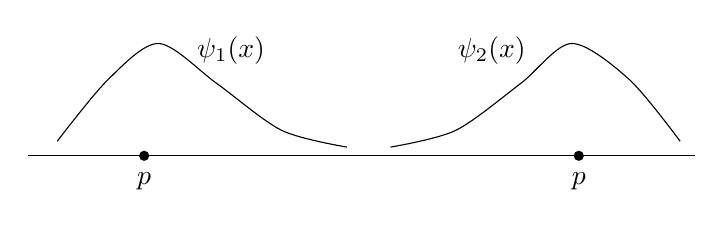
\begin{tikzpicture}[scale=0.92]
\draw (-0.2,0) -- (9.0,0);
\fill (1.4,0) circle (2pt);
\fill (7.4,0) circle (2pt);
\draw[smooth] plot coordinates {(0.2,0.2) (0.9,1.05) (1.6,1.55) (2.4,1.0) (3.3,0.35) (4.2,0.12)};
\draw[smooth] plot coordinates {(4.8,0.12) (5.7,0.35) (6.6,1.0) (7.3,1.55) (8.1,1.05) (8.8,0.2)};
\node at (1.4,-0.35) {$p$};
\node at (7.4,-0.35) {$p$};
\node at (2.6,1.45) {$\psi_1(x)$};
\node at (6.2,1.45) {$\psi_2(x)$};
\end{tikzpicture}
\caption{在允许隧穿后，用于形成平衡叠加态的两个局域剖面。}
\lectureframe{00:17:54}
\end{figure}
\editorialnote{标签\(\psi_1(x)\)和\(\psi_2(x)\)标识了在00:17:41--00:17:56处所讨论的两个剖面；这些符号是为了便于辨认而添加的示意性标签。}

在无穷远分隔时，这两个态是简并的：把电子局域在左侧或右侧所付出的能量相同。在有限分隔时，一种新过程成为可能。电子可以从一个中心隧穿通过经典禁戒区到达另一个中心。若去观察一条穿过势垒的轨迹，就会扰动该态；``跳跃''是对量子演化的描述，而不是经典路径的影片。

在平衡时，电子在任一质子附近被找到的概率相等。因此归一化给出因子\(1/\sqrt2\)，而较低的平衡态近似为
\begin{equation}
\psi_+(x)\approx \frac{\psi_1(x)+\psi_2(x)}{\sqrt2}.
\end{equation}

近似号很重要。真正的双中心波函数并不严格是两个未受扰动的类氢轨道的和；它会在重叠区发生调整。这里所需的要点是，对称的平衡态位于孤立的一中心能量之下。用哈密顿量的语言说，左、右两种组态由一个非对角矩阵元耦合。允许电子占据它们的相干叠加降低了能量。

\section{从能量降低到有效力}

在质子间距很大时，电子诱导的贡献\(E_e(r)\)趋近其分离原子值。在较小的间距下，隧穿和叠加使它降低。完整的两质子--单电子势还必须包含质子间的直接排斥，
\begin{equation}
V_{\mathrm{tot}}(r)=V_{pp}(r)+E_e(r).
\end{equation}

这使分子例子与场能论证重新联系起来。波函数草图与\(E_e(r)\)的定性曲线是同一计算的两种视图；平衡由总和\(V_{\mathrm{tot}}(r)\)决定。

\begin{figure}[h]
\centering
\includegraphics[width=0.78\textwidth]{lecture_01_figure_04.png}

\medskip

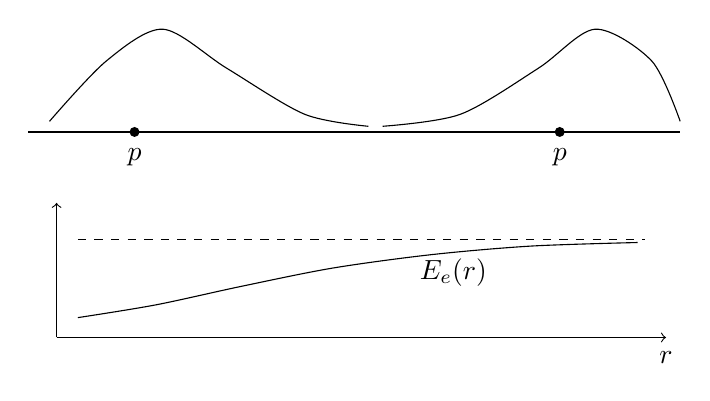
\begin{tikzpicture}[scale=0.9]
\draw (-0.2,3.0) -- (9.0,3.0);
\fill (1.3,3.0) circle (2pt);
\fill (7.3,3.0) circle (2pt);
\draw[smooth] plot coordinates {(0.1,3.15) (0.9,4.0) (1.7,4.45) (2.6,3.9) (3.7,3.25) (4.6,3.08)};
\draw[smooth] plot coordinates {(4.8,3.08) (5.9,3.25) (7.0,3.9) (7.8,4.45) (8.6,4.0) (9.0,3.15)};
\node at (1.3,2.65) {$p$};
\node at (7.3,2.65) {$p$};

\draw[->] (0.2,0.1) -- (0.2,2.0);
\draw[->] (0.2,0.1) -- (8.8,0.1);
\draw[dashed] (0.5,1.48) -- (8.5,1.48);
\draw[smooth] plot coordinates {(0.5,0.38) (1.6,0.56) (2.8,0.82) (4.1,1.08) (5.5,1.27) (6.9,1.39) (8.4,1.44)};
\node at (5.8,1.02) {$E_e(r)$};
\node at (8.8,-0.18) {$r$};
\end{tikzpicture}
\caption{上方为波函数重叠，下方为电子诱导的能量。随着\(r\)增大，它向分离原子渐近值上升；质子总势还必须包含它们之间的库仑排斥。}
\lectureframe{00:20:28}
\end{figure}
\editorialnote{标签\(E_e(r)\)和\(r\)标识了在00:19:12--00:20:38处所讨论的能量曲线和间距；保留下来的板书画面并不能使那些坐标轴标签变得可辨认。}

相应的两个力由能量梯度给出，
\begin{equation}
F_{e}(r)=-\frac{dE_e}{dr},
\qquad
F_{\mathrm{tot}}(r)=-\frac{dV_{\mathrm{tot}}}{dr}.
\end{equation}
因此系统被推向更低的总能量。在\(E_e(r)\)随质子接近而减小的区域，交换提供吸引性贡献；是否存在束缚间距取决于它与\(V_{pp}(r)\)的竞争。这就是共价键背后的基本机制：电子之所以被共享，是因为共享态在能量上有利。

在经典计算中，电场的重叠改变能量。在这里，两个力心允许一个更低的量子态。两种机制都产生力，因为平衡能量依赖于组态。

交换的语言可以用世界线草图来概括。它不能被解读为被观测到的轨迹；它表示电子与任一质子相关联的振幅。

\begin{figure}[h]
\centering
\begin{tikzpicture}[scale=1.0]
\draw (0,0) -- (0,4.4);
\draw (4.8,0) -- (4.8,4.4);
\draw (0,0.9) .. controls (1.6,1.7) and (3.2,1.7) .. (4.8,2.5);
\draw (4.8,2.9) .. controls (3.2,2.1) and (1.6,2.1) .. (0,3.9);
\node at (0,-0.35) {$p$};
\node at (4.8,-0.35) {$p$};
\node at (2.35,1.55) {$e^-$};
\node at (2.35,2.55) {$e^-$};
\end{tikzpicture}
\caption{两个质子世界线之间的电子交换，应理解为量子振幅的示意图，而不是被观察的路径。}
\end{figure}

\begin{classroomqa}
\audiencequestion{这种吸引能否简单地理解为电子对质子电荷的屏蔽或削减？\lecturetimestamp{00:23:26}}
\lecturerresponse{不能。电荷削减并不是描述这一效应的正确图像。关键事实在于，将两个定域波函数相加所产生的态，其能量略低于两个定域态各自单独存在时的能量。}
\end{classroomqa}

\begin{classroomqa}
\audiencequestion{这是否就是费曼所说的``光喜欢光''的意思？\lecturetimestamp{00:23:51}}
\lecturerresponse{不是。那句话最可能涉及的是玻色统计：光子倾向于占据共同状态，而电子则服从不相容原理。这里的分子效应是电子在两个中心之间的隧穿。}
\end{classroomqa}

两个质子之间仍然存在静电排斥。交换作用的力程比库仑相互作用更短，因此必须考虑总势能，而不能只看其中任一贡献。在适当的间距下，分子离子\(\mathrm H_2^+\)仍然是束缚的；在中性双电子体系中，长程电荷排斥不存在，共价结合就更为常见。

\begin{classroomqa}
\audiencequestion{把电子放在两个质子之间，主要是减小了它们之间的静电排斥吗？\lecturetimestamp{00:24:33}}
\lecturerresponse{它确实会略微减小排斥，但这不是主要效应。电子交换是一种比库仑排斥力程更短的力。它在中性双电子体系中最为明显，因为此时原子之间的长程静电力不存在，而隧穿仍然产生吸引。}
\end{classroomqa}

\begin{classroomqa}
\audiencequestion{带正电、只有一个电子的分子离子\(\mathrm H_2^+\)真的束缚吗？\lecturetimestamp{00:26:06}}
\lecturerresponse{是的。在足够小的间距下，交换吸引足以克服质子--质子之间的库仑排斥。}
\end{classroomqa}

\begin{classroomqa}
\audiencequestion{双中心排布是否产生了一种第三种力？\lecturetimestamp{00:26:24}}
\lecturerresponse{并没有引入新的基本力。两个质子的合成势场中的Schr\"odinger方程，其平衡能量不同于单中心问题；这一改变了的能量的导数就是有效力。}
\end{classroomqa}

\begin{classroomqa}
\audiencequestion{能量降低是量子纠缠的一个例子吗？\lecturetimestamp{00:27:06}}
\lecturerresponse{不是通常双粒子意义上的纠缠：这里只需要一个电子。相关的数学特征是耦合左右两个态的非对角哈密顿矩阵元。}
\end{classroomqa}

\begin{classroomqa}
\audiencequestion{高温下交换会怎样？\lecturetimestamp{00:27:37}}
\lecturerresponse{在极端温度下，电子被电离，完全不再记得这个分子。在较低的激发能量下，它可能占据一个更大的轨道，从而改变重叠，进而改变力。这是一种依赖于状态的修正，而不是一种新的普遍机制。}
\end{classroomqa}

\section{光子交换与表中的最初几项}

库仑力能否用同样的交换语言来描述？带电粒子与电磁场相互作用，而电磁场的量子就是光子。经典地，我们求解电荷周围的电场。在量子场论中，我们把这种相互作用分解为光子的发射与吸收。

一个物理带电粒子并不只是一个裸电荷。它的态是一种量子叠加，包含裸电子分量、带一个光子的电子、带两个光子的电子，依此类推。用刻意示意性的记号表示，
\begin{equation}
\begin{aligned}
\ket{e_{\mathrm{phys}}}
={}&a_0\ket e
+a_1\ket{e+\text{one photon}}
\\
&+a_2\ket{e+\text{two photons}}+\cdots .
\end{aligned}
\end{equation}
这种记号只记录了光子数分量的层级；它并未指定光子的动量，也没有试图完整构造一个相互作用的带电态。
周围的光子是被发射和再吸收的，而不是作为自由辐射逃逸出去。它们的效应可以被测量，尽管其探测方式与自由传播的光子不同。在附近放置第二个电荷，一个电荷处发射的光子就可以被另一个电荷吸收。于是这两个缀饰态的能量就不再等于两个孤立能量之和。

课堂上的类比是两个杂耍者，各自抛接一组球。当他们相距很远时，各自独立地抛接。把他们拉得足够近，一个人就可能接住另一个人抛来的球。用费曼图的语言来说，那个被共享的对象就是被交换的光子。这个类比并不是微观轨迹，但它抓住了为什么靠近会允许一种新过程发生。

现在我们有了两种超越单纯记忆库仑定律的描述。经典场论把场相加并将结果平方。量子场论则对交换量子的振幅求和。在这个意义上，粒子、场和力构成一一对应的关系。电子传递分子交换，光子传递电磁交换，而任何能够被交换的粒子在适当情境下都能对力作出贡献。因此，那个熟悉的说法——自然界有四种基本相互作用——是一种更宏观层面上的分类；在交换语言中，每一种可交换的粒子种类都能产生其自身的有效力贡献。

现在终于到了给粒子命名、列出它们的性质、并说明它们能参与哪些过程的时候了。一次性写出整个标准模型只会变成一场冗长的记忆测试，所以我们将把粒子分成若干小组，使组内成员彼此有简单关联，并逐一了解每一组能做什么。

完整的目录之所以繁琐，是因为我们并不理解为什么恰恰是这些粒子存在，而其他可以想象的粒子却不存在。数学自洽性提供了一些关系：一旦某个模式中的若干成员存在，就可能需要另一个成员来补全它。这些关系减少了独立事实的数目，但只减少了一个不大的因子。许多粒子种类和许多参数仍然得不到解释。理解这一未完成的结构，对于理解后来的实验试图发现什么，是必要的。

\begin{figure}[h]
\centering
\includegraphics[width=0.7\textwidth]{lecture_01_figure_05.png}
\caption{粒子表的第一项通过\(\gamma\)标识光子，并通过矢量势\(A\)标识其场。}
\lectureframe{00:39:11}
\end{figure}

第一个场--量子的对应关系是
\begin{equation}
\gamma \leftrightarrow A.
\end{equation}
这里\(A\)是电磁矢量势。光子是自旋为1的玻色子，其电荷为零、重子数为零、静止质量为零。电子场按惯例记作\(\psi_e\)；它的产生和湮灭部分作用于电子态和正电子态。

我们的表格记录了名称、粒子符号、场、玻色子或费米子类型、电荷\(Q\)、重子数\(B\)和质量：

\begin{table}[h]
\centering
\resizebox{\linewidth}{!}{%
\begin{tabular}{lllllll}
名称&符号&场&类型&\(Q\)&\(B\)&质量\\
光子&\(\gamma\)&\(A\)&玻色子&\(0\)&\(0\)&\(0\)\\
电子&\(e^-\)&\(\psi_e\)&费米子&\(-1\)&\(0\)&\(0.51\,\mathrm{MeV}\)\\
正电子&\(e^+\)&\(\psi_e\)&费米子&\(+1\)&\(0\)&\(0.51\,\mathrm{MeV}\)
\end{tabular}
}%
\caption{作为粒子目录开头的光子和电子--正电子条目。}
\end{table}

电子与正电子之间的关系是相互的：每一个都是另一个的反粒子。把带负电的态``称为粒子''是一种约定。我们以电子电荷的绝对值为单位来测量电荷，因此
\begin{equation}
Q(e^-)=-1,\qquad Q(e^+)=+1.
\end{equation}
质量通过使用\(E=mc^2\)以能量单位来测量。一个电子伏特是电荷\(e\)经过一伏特电势差所获得的能量，
\begin{equation}
1\,\mathrm{eV}=e\,(1\,\mathrm V).
\end{equation}
这个单位自然地来自原子物理：作为粗略的原子尺度，电离氢大约需要\(13.5\,\mathrm{eV}\)。粒子质量则需要数百万或数十亿电子伏特。电子质量为
\begin{equation}
m_e c^2 \approx 0.511\,\mathrm{MeV}.
\end{equation}

\begin{classroomqa}
\audiencequestion{电子质量是否恰好是MeV的一半？\lecturetimestamp{00:44:02}}
\lecturerresponse{不是。方便的取整值\(0.51\,\mathrm{MeV}\)并非由任何原理固定为精确的一半；它是一个测量得到的参数。}
\end{classroomqa}

基本的QED过程有一条带电费米子线进入、一条离开，并附有一条光子线。重新排列或交叉这些腿，可以让同一个顶点描述光子的发射、吸收或正电子过程。在这里使用的非协变示意记法中，相互作用包含
\begin{equation}
\mathcal{L}_{\mathrm{int}}\sim e\,\psi_e^\dagger \psi_e A.
\end{equation}
将场展开为产生和湮灭算符，会产生这样的项：它们移除一个入射电子、产生一个出射电子，并产生或湮灭一个光子。耦合\(e\)在顶点处提供一个因子。因此，对于电子被散射或加速时的光子发射，
\begin{equation}
\mathcal{A}_{\mathrm{vertex}}\propto e,
\qquad
P_{\mathrm{emission}}\propto e^2.
\end{equation}
在X射线管中，电子撞击靶是这种光子发射概率起作用的一个实际情境。同一个顶点的反复组合产生了量子电动力学的各种过程，包括被解释为电荷之间作用力的能量移动。

因此，一个示意性的顶点是有用的。

\begin{figure}[h]
\centering
\begin{tikzpicture}[scale=1.0]
\fill (0,0) circle (1.5pt);
\draw (-1.6,-1.2) -- (0,0) -- (1.6,-1.2);
\draw (0,0) -- (0,1.8);
\node at (-1.8,-1.4) {$e^-$};
\node at (1.8,-1.4) {$e^-$};
\node at (0.35,1.95) {$\gamma$};
\end{tikzpicture}
\caption{基本QED顶点的拓扑示意图：一条带电费米子线进入，一条离开，并附着一个光子。此处笔直的光子腿只是简化的绘图约定。}
\end{figure}

力的交换贡献将两个这样的顶点连接起来：

\begin{figure}[h]
\centering
\begin{tikzpicture}[scale=1.0]
\draw (0,0) -- (0,4.0);
\draw (4.8,0) -- (4.8,4.0);
\draw (0,2.0) -- (4.8,2.0);
\node at (0,-0.35) {$e^-$};
\node at (4.8,-0.35) {$e^-$};
\node at (2.4,2.3) {$\gamma$};
\end{tikzpicture}
\caption{光子交换的拓扑示意图，给出库仑相互作用的量子场论描述。}
\end{figure}

粒子--场--力这个三角形闭合之后，我们可以继续这份目录。

\section{夸克、重子数与代之谜}

如果这份目录写于1960年前后，那么质子和中子很可能会紧随电子和光子之后。现代粒子物理学则把夸克放在最前面。在朴素的组分图像中，质子和中子是相对较大的复合体，由更小的夸克自由度构成。\emph{复合}的确切含义仍有待考察，但组分的语言已经极其有用。

所有夸克都是费米子。它们携带重子数，这是核物理学中通过计数核子引入的一个量。\emph{核子}特指质子或中子。\emph{重子}是更广的一类，包含核子以及后来遇到的类似重粒子。质子和中子各自具有一个单位，
\begin{equation}
B(p)=B(n)=1,
\qquad
B(\bar p)=B(\bar n)=-1.
\end{equation}
对于原子核，这个重子计数恰好就是质量数\(A=Z+N\)，即质子数加中子数。以原子质量单位测得的数值原子质量只是近似等于\(A\)。在{\proseunicodefont β}过程中，质子可以变成中子，中子也可以变成质子，但核子的总数不变。例如，
\begin{equation}
n\longrightarrow p+e^-+\bar\nu_e
\end{equation}
分别改变了质子数和中子数，同时保持它们的和不变。

\begin{classroomqa}
\audiencequestion{同位素是否与质子数加中子数守恒相矛盾？\lecturetimestamp{00:52:03}}
\lecturerresponse{不同的同位素确实含有不同的中子数，而{\proseunicodefont β}衰变可以使一个中子与一个质子互换。在普通的核过程中，相关的守恒计数是总重子数，而不是任一粒子种类的数目。}
\end{classroomqa}

归一化是约定俗成的。我们本可以给质子指定重子数\(2\)、\(7\)或\(\pi\)，只要每个复合体都一致地缩放即可。一旦给质子指定\(B=1\)并且它包含三个夸克，每个夸克就必须携带
\begin{equation}
B(q)=\frac13,
\qquad
B(\bar q)=-\frac13.
\end{equation}
因此，这个分数值是先对复合核子进行归一化所造成的历史性后果。

\begin{classroomqa}
\audiencequestion{夸克数是守恒的吗？\lecturetimestamp{00:54:23}}
\lecturerresponse{夸克--反夸克对可以被产生或湮灭，所以原始的数目并不守恒。对应于重子数的量是夸克数减去反夸克数，再除以三。经验上它以极高的精度守恒，尽管这里并不假定它是一条绝对定律。}
\end{classroomqa}

一个假想的电荷守恒衰变，例如
\begin{equation}
p\longrightarrow e^++\gamma
\end{equation}
会把重子数为一的初态变成一个重子数为零的末态。这个道只是一个说明性的记账例子，而不是一个被提出的衰变模型。尚未观察到任何破坏重子数的过程。这里引用的粗略界限把质子寿命至少置于\(10^{33}\)--\(10^{34}\)年的范围内。人们不会对单个质子观察那么久；而是对数量巨大的质子观察一段可管理的时间，用寿命与样本大小作交换。尽管如此，质子衰变曾被广泛预期，而这里所讨论的数学中没有任何东西提供绝对的禁止。因此，重子数是否严格守恒仍然是一个悬而未决的实验问题：未被观察到，受到强烈限制，但并未被排除。

\begin{classroomqa}
\audiencequestion{质子--反质子湮灭是否违反重子数？\lecturetimestamp{00:56:17}}
\lecturerresponse{不违反。初始重子数为\(1+(-1)=0\)，因此湮灭到重子数为零的末态是守恒的。一个孤立的质子衰变成非重子产物才会是违反。}
\end{classroomqa}

有六种夸克味，
\begin{equation}
u,\ d,\ s,\ c,\ b,\ t,
\end{equation}
称为上、下、奇异、粲、底和顶。上夸克并没有什么指向上方的性质，奇异夸克也不比它的邻居更奇异；这些名称记录的是历史而非逻辑。场的记号并不完全统一：人们会遇到\(q\)、\(Q\)、\(\psi_q\)，或者干脆用味字母\(u,d,s,c,b,t\)来同时表示场及其量子。

\begin{classroomqa}
\audiencequestion{底夸克和顶夸克就是曾经被称为美夸克和真夸克的同一种粒子吗？\lecturetimestamp{00:58:35}}
\lecturerresponse{是的。较为朴素的名称底夸克和顶夸克成为了标准名称。命名的历史不包含任何动力学内容。}
\end{classroomqa}

它们的电荷以三对的形式重复：
\begin{equation}
\begin{aligned}
Q(u)=Q(c)=Q(t)&=+\frac23,
\\
Q(d)=Q(s)=Q(b)&=-\frac13.
\end{aligned}
\end{equation}
反夸克带有相反的电荷和重子数。孤立的分数电荷从未被观测到，因为夸克不会以自由渐近粒子的形式出现；观测到的强子具有整数电荷。

\((d,u)\)、\((s,c)\)和\((b,t)\)这三对是重复相同电荷模式的三代。全部六种夸克仍然带有\(B=1/3\)。

\begin{classroomqa}
\audiencequestion{较重的夸克是否也带有重子数\(1/3\)？\lecturetimestamp{01:02:02}}
\lecturerresponse{是的。每一种夸克都带有重子数\(1/3\)。}
\end{classroomqa}

质量则没有显示出可与之相比的重复性。有用的数量级数值为
\begin{align}
m_u &\sim 5\,\mathrm{MeV},
&
m_d &\sim 10\,\mathrm{MeV},
\\
m_s &\sim 100\,\mathrm{MeV},
&
m_c &\sim 10^3\,\mathrm{MeV},
\\
m_b &\sim 5\,\mathrm{GeV},
&
m_t &\sim 170\,\mathrm{GeV}.
\end{align}
这里\(1\,\mathrm{GeV}=10^3\,\mathrm{MeV}\)；单位的改变使底夸克和顶夸克的条目保持可读。下夸克的估计值远高于电子的\(0.511\,\mathrm{MeV}\)，但远低于质子的约\(940\,\mathrm{MeV}\)，约为\(1{,}800\)个电子质量。事实上，把两个轻的上夸克条目和一个下夸克条目相加，远不能达到质子质量；强子能量的其余部分最终必须得到解释。

\editorialnote{口头比较中把一个\(10\,\mathrm{MeV}\)的下夸克说成约五十个电子质量。用这里写出的粗略数值，\(10/0.511\approx20\)；层级关系是正确的，但五十这个因子是算术失误。}

甚至一对之内的顺序也没有重复：下夸克比上夸克重，而粲夸克比奇异夸克重得多。顶夸克比上夸克重数万倍，尽管它们的电荷和相互作用模式非常相似。

这里实际上有两个谜题。我们不理解为什么甚至存在一个夸克代，尽管第一代至少提供了质子和中子以及普通物质所需的上夸克和下夸克。我们也不理解为什么自然界在第二代和第三代中重复这一模式，或者为什么重复出现的粒子质量散布在如此多的数量级上。有一些想法，但还没有被接受的解释能够计算出这一模式。

\begin{classroomqa}
\audiencequestion{如果顶夸克质量没有根本性的解释，那么在直接发现之前，它的近似值是如何被预言的？\lecturetimestamp{01:05:53}}
\lecturerresponse{这一估计并不是从更深层的原理推导出质量。人们假定一个候选质量，计算虚顶夸克影响已精确测量过程的图，并询问哪个值与那些观测一致。间接敏感性可以定位一个参数，而不解释自然界为什么选择它。}
\end{classroomqa}

\begin{classroomqa}
\audiencequestion{如果自由夸克不能被孤立出来，那么在什么意义上可以说夸克被探测到了？\lecturetimestamp{01:08:04}}
\lecturerresponse{夸克的证据是可探测的：它们的产生留下特征性的能量、方向和粒子喷注，而虚夸克影响其他可观测量。不能制备的是一个与所有强子伴粒子分离、并作为孤立渐近粒子加以考察的单独夸克。}
\end{classroomqa}

\begin{classroomqa}
\audiencequestion{电荷\(-1/3\)和\(+2/3\)的模式是从理论推导出来的，还是仅仅是一种记账？\lecturetimestamp{01:09:02}}
\lecturerresponse{这一模式的一部分是数学一致性所要求的，但只是一部分。在这个阶段，电荷是作为事实被记录下来的；一致性条件只有在标准模型的更多内容就位之后才会讨论。}
\end{classroomqa}

只有\(u\)和\(d\)夸克在普通物质中具有可观的丰度。较重的味衰变到较轻的状态。因此，上夸克和下夸克的相对丰度在很大程度上由质子和中子的宇宙丰度和核丰度以及它们的组分含量决定。

\begin{classroomqa}
\audiencequestion{是什么决定了宇宙中六种夸克味的相对丰度？\lecturetimestamp{01:09:49}}
\lecturerresponse{稳定物质基本上只包含上夸克和下夸克；较重的味会衰变。自由中子会衰变，而质子在观测时间尺度上是稳定的，尽管中子在束缚于原子核中时仍然大量存在。在这个层面上，数上夸克和下夸克就归结为数那些质子和中子。}
\end{classroomqa}

\section{从夸克到强子：核子、奇异重子和介子}

一旦夸克电荷已知，熟悉的强子就可以重新构建。中子和质子各包含三个价夸克，
\begin{equation}
n=ddu,
\qquad
p=uud.
\end{equation}
它们的电荷立即得到验证：
\begin{align}
Q(n) &= Q(d)+Q(d)+Q(u)
= -\frac13-\frac13+\frac23
=0,\\
Q(p) &= Q(u)+Q(u)+Q(d)
= \frac23+\frac23-\frac13
=1.
\end{align}

暂时忘掉光子。把电磁相互作用关掉后，质子和中子看起来几乎就是同一个物体，只是\(u\)和\(d\)互换而已。这种近似对称并不精确，因为这两种夸克的质量并不完全相等。我们要等到遇见相应的轻介子之后，才会命名并展开这一对称性。

由于\(m_d>m_u\)，含有两个下夸克的中子应当获得更大的夸克质量贡献。电磁自能则朝相反方向推动：带电的质子储存电场能量，而中子没有净电荷。自然界以中子略重的方式解决了这一竞争。在这种粗略近似下，
\begin{align}
m_pc^2&\approx940\,\mathrm{MeV},\\
m_nc^2&\approx940\,\mathrm{MeV},\\
(m_n-m_p)c^2&\approx1.4\,\mathrm{MeV}.
\end{align}

\begin{classroomqa}
\audiencequestion{质子和中子的质量是多少？\lecturetimestamp{01:15:35}}
\lecturerresponse{在这种粗略程度上，两者都接近\(940\,\mathrm{MeV}\)，相差约\(1.4\,\mathrm{MeV}\)。}
\end{classroomqa}

然而，这一微小的过剩已足以允许自由中子衰变。在支付电子静止能量之后，剩余能量可以作为动能出现在\(n\to p+e^-+\bar\nu_e\)中。

同样的组分逻辑会产生奇异重子。由于\(s\)和\(d\)具有相同的电荷，可以用奇异夸克替换下夸克而不改变电荷模式：
\begin{equation}
uds,\qquad uss,\qquad uus.
\end{equation}
因此在上面的例子中，\(uds\)和\(uss\)是中性的，而\(uus\)的电荷为\(+1\)。这类态获得了包括\(\Lambda\)和\(\Xi\)在内的名称；现阶段无需对这些名称作详细指派。把\(d\)替换为\(s\)，在定性上类似于在相关原子核中用一种核子替换另一种核子：大部分结合模式保持不变，而组分的改变使质量发生移动。这些态比普通核子重，并衰变为较轻的重子，同时伴随为携带能量和其他守恒量子数所需的任何额外粒子。

\begin{classroomqa}
\audiencequestion{奇异重子衰变时会出现什么？\lecturetimestamp{01:19:02}}
\lecturerresponse{会出现质子或中子这样的较轻重子，但它不可能是唯一的产物：多余的能量和守恒量子数要求有额外粒子。详细的衰变规则留待以后讨论。}
\end{classroomqa}

详细的替换规则比这份初步目录更复杂，但一种安全的操作是把一种味替换为具有相同电荷的另一种味。在这种粗略的组分层面上，把下夸克替换为奇异夸克大约增加\(90\,\mathrm{MeV}\)。因此这些重子比质子和中子稍重。由于它们可以衰变为较轻的核子，所以它们在我们周围的普通物质或宇宙中并不丰富。

\begin{classroomqa}
\audiencequestion{是否每个重子都有一个反重子，由把每个夸克替换为其反夸克得到？\lecturetimestamp{01:20:33}}
\lecturerresponse{是的。把每个组分替换为其反粒子，就产生反质子、反中子或相应的反奇异重子，所有可加电荷都反号。}
\end{classroomqa}

\begin{classroomqa}
\audiencequestion{如果把奇异夸克替换为底夸克，又会怎样？\lecturetimestamp{01:21:00}}
\lecturerresponse{结果是一个底重子。``奇异重子''特指存在一个\(s\)夸克；这个形容词命名的是味，而不是一般意义上的陌生程度。}
\end{classroomqa}

形容词\emph{奇异}是在物理学家已经熟悉质子和中子、而新发现的粒子在它们旁边显得出乎意料之后才出现的。一旦知道了味结构，它们的存在就不比任何其他夸克复合体更奇异。

组分质量暴露出一个重要警告。把两个上夸克质量和一个下夸克质量相加，只得到几十MeV，远不及质子的大约\(940\,\mathrm{MeV}\)。那个朴素求和遗漏了某些实质性的东西。质子和中子还含有胶子，而胶子携带能量。在相对论性束缚系统中，复合体的质量并不是简单地把其组分的所列质量相加就能得到的。

\begin{classroomqa}
\audiencequestion{质子和中子那看似缺失的质量来自哪里？胶子携带质量吗？\lecturetimestamp{01:21:26}}
\lecturerresponse{在这种记账中，胶子不携带重子数，但它们确实携带能量。它们的能量正是质子和中子的质量不等于轻夸克质量项之和的部分原因。}
\end{classroomqa}

\begin{classroomqa}
\audiencequestion{那部分缺失的贡献是一种结合能吗？\lecturetimestamp{01:22:03}}
\lecturerresponse{是的，可以称之为一种结合能。警告在于：相对论性复合体的质量并不像把组分质量参数相加所暗示的那样简单相加。}
\end{classroomqa}

\begin{classroomqa}
\audiencequestion{复合质子能否像用粒子语言那样，也用场的语言来描述？\lecturetimestamp{01:22:45}}
\lecturerresponse{可以，但要困难得多。对于这里正在建立的组分记账方式而言，粒子语言远比试图直接组合空间上延展的场要透明得多。}
\end{classroomqa}

\begin{classroomqa}
\audiencequestion{普通结合能相对于分离的组分是负的。为什么核子的动力学贡献却是一个大的正能量？\lecturetimestamp{01:23:32}}
\lecturerresponse{通常的负结合能直觉在这种情况下并不成立。其解释属于后面关于强相互作用的讨论，所以这个问题暂时搁置。}
\end{classroomqa}

为什么三个夸克形成重子，而两个夸克却不形成孤立的双夸克强子？在夸克理论的早期，这确实是一个真正的谜题。人们可能会回答说，所观测到的束缚组合必须具有等于电子电荷整数倍的电量。仅凭这一点听起来是循环论证：它描述了这一模式，却没有解释它。尽管如此，这条规则后来证明是指向了正确的方向，而其更深层的起源只有在强相互作用的理论建立得更多之后才能理解。就目前而言，它明确是一条工作规则：三个夸克可以构成一个重子，而一个夸克和一个反夸克可以构成一个介子，由此得到的观测复合粒子具有整数电荷。

由三个相同轻味组成的重子也会出现，但其细节可以等到介子之后再讨论。

介子是\(q\bar q\)复合粒子。它们的重子数消失，
\begin{equation}
B(q\bar q)=\frac13-\frac13=0.
\end{equation}
最轻的例子使用\(u\)和\(d\)。这些味比其他味轻得多，在普通物质中稳定或消失得相对缓慢，并且在自然界中丰度很高。它们的产生阈值低，也意味着碰撞比产生重味更容易产生它们。由于所有这些原因，轻夸克复合粒子是实验上最早遇到的介子，也是自然的起点。

自然的味基是
\begin{equation}
\ket{\bar u d},\qquad \ket{u\bar d},\qquad \ket{\bar u u},\qquad \ket{\bar d d}.
\end{equation}
在这第一次计数中没有使用额外的限制：所有四种轻夸克--反夸克配对都被保留，然后计算它们的电荷。

带电态是直接的。由于\(Q(\bar u)=-2/3\)和\(Q(d)=-1/3\)，
\begin{align}
Q(\bar u d)&=-\frac23-\frac13=-1,
&
\ket{\pi^-}&=\ket{\bar u d}.
\end{align}
把每个组分替换为其反粒子就得到\(u\bar d\)，所以第二个态是第一个态的反粒子：
\begin{align}
Q(u\bar d)&=+\frac23+\frac13=+1,
&
\ket{\pi^+}&=\ket{u\bar d}.
\end{align}

同味态是中性的，但其中任何一个本身都没有单独的粒子名称。量子力学允许我们将它们叠加。两个归一化、正交的组合是
\begin{align}
\ket{\pi^0} &\approx \frac{\ket{\bar u u}-\ket{\bar d d}}{\sqrt2},\\
\ket{\eta} &\approx \frac{\ket{\bar u u}+\ket{\bar d d}}{\sqrt2}.
\end{align}

\begin{figure}[h]
\centering
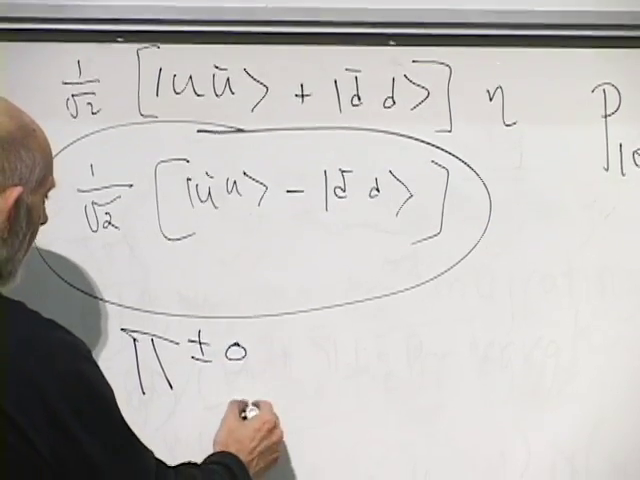
\includegraphics[width=0.82\textwidth]{lecture_01_figure_06.png}
\caption{对称的中性组合被认定为\(\eta\)，而反对称组合则与{\proseunicodefont π}介子三重态归为一组。}
\lectureframe{01:32:35}
\end{figure}

每个中性态都是一个纠缠的夸克--反夸克对，不是通过普通自旋，而是通过\emph{上性}和\emph{下性}。如果把上味和下味在数学上像自旋半变量的两个方向那样处理，那么上面的和与差就扮演与熟悉的两自旋叠加相同的角色。这种自旋的内部类比称为\emph{同位旋}。没有任何东西在空间中字面地指向上或下；这两个方向标记的是\(u\)和\(d\)味。

三个{\proseunicodefont π}介子\(\pi^+\)、\(\pi^0\)和\(\pi^-\)构成一个同位旋三重态。它们的质量几乎相等，如果上夸克和下夸克的质量完全相同，它们会更加接近。正交的中性态称为\(\eta\)。

\(\eta\)比{\proseunicodefont π}介子重得多：
\begin{equation}
m_\pi \approx 140\,\mathrm{MeV},
\qquad
m_\eta \approx 500\,\mathrm{MeV}.
\end{equation}
为什么\(\eta\)与众不同，长期以来一直不清楚。现在这一解释已经理解，但它在数学上很抽象，这里不展开。

\begin{classroomqa}
\audiencequestion{这些介子相对长寿命吗？\lecturetimestamp{01:33:59}}
\lecturerresponse{相对于许多强衰变粒子而言，是的。在所讨论的通道中，它们不通过强相互作用衰变；弱衰变和电磁衰变使它们寿命更长。}
\end{classroomqa}

\begin{classroomqa}
\audiencequestion{各个中性态\(\bar u u\)和\(\bar d d\)有它们自己的名称吗？\lecturetimestamp{01:34:29}}
\lecturerresponse{没有。被命名的粒子是由它们的和与差形成的线性组合；那些组合具有确定的值。}
\end{classroomqa}

\begin{classroomqa}
\audiencequestion{这种中性态叠加是否类似于中微子振荡？\lecturetimestamp{01:34:44}}
\lecturerresponse{在有限的意义上相似，因为两者都涉及量子叠加。这里的问题更密切地关系到两个自旋为二分之一的组分的自旋组合，以及这类态可以纠缠的两种方式。这一讨论留待下一讲。}
\end{classroomqa}

一旦引入奇异夸克，将\(d\)或\(\bar d\)替换为\(s\)或\(\bar s\)，就得到四个奇异或\(K\)介子味态
\begin{equation}
\bar u s,\qquad u\bar s,\qquad \bar d s,\qquad d\bar s.
\end{equation}
它们的电荷分配为
\begin{align}
Q(\bar u s) &=-1,
&
Q(u\bar s) &=+1,
\\
Q(\bar d s) &=0,
&
Q(d\bar s) &=0.
\end{align}
因此有两个带电K介子和两个中性K介子。

第一次计数给出三个{\proseunicodefont π}介子、四个K介子和一个\(\eta\)：八个态。但该列表尚未使用\(\ket{s\bar s}\)配对。由于有三种味和三种反味，完整的基本计数因此为
\begin{equation}
3\times3=9.
\end{equation}
缺失的\(s\bar s\)态补全了九个夸克--反夸克味组合的计数。
